% ----------------------------------------------------------
\chapter{Revisão Bibliográfica}\label{cap:revisaobibliografica}
% ----------------------------------------------------------

% ----------------------------------------------------------
\section{Definições}
% ----------------------------------------------------------

No intuito de esclarecer termos e conceitos utilizados neste trabalho, dedica-se esta seção.

% ----------------------------------------------------------
\subsection{Resíduos Sólidos Industriais}
% ----------------------------------------------------------

De acordo com o \gls{PNRS}, resíduos sólidos são todo:

\begin{citacao}
	"Material, substância, objeto ou bem descartado resultante de atividades humanas em sociedade, cuja destinação final se procede, se propõe proceder ou se está obrigado a proceder, nos estados sólido ou semissólido, bem como gases contidos em recipientes e líquidos cujas particularidades tornem inviável o seu lançamento na rede pública de esgotos ou em corpos d’água, ou exijam para isto soluções técnicas ou economicamente inviáveis em face da melhor tecnologia disponível. \cite[Art. 3º, ítem XVI]{brasil_lei_nodate}"		
\end{citacao}

No contexto deste trabalho, considera-se em especial \gls{RSI}s, conforme mencionado no website do \gls{SINIR} como: resíduos gerados nos processos produtivos e instalações industriais \cite{sinir_sinir_nodate}.

% ----------------------------------------------------------
\subsection{Direcionamento de resíduos sólidos industriais}
% ----------------------------------------------------------

Em consonância com a seção V do \gls{PNRS} que responsabiliza os geradores de resíduos enquandrados nas alíneas  “e”, “f”, “g” e “k” do inciso I do art. 13 — sendo “f” relativa aos geradores de \gls{RSI}s — a elaborarem o \gls{PGRS}, o qual aponta e descreve as ações realizadas para minimizar a geração de resíduos na fonte e procedimentos relacionados à movimentação dos resíduos até que cheguem à destinação ambientalmente adequada.

A \autoref{fig:Fig_1} ilustra as principais destinações finais de resíduos em \gls{SC} por município. É possível observar a ausência de lixões em todo estado, bem como a vasta quantidade de aterros sanitários, ambos indicativos de uma boa condução no que tange a descarte de resíduos.

Apesar de não termos lixões no estado, entende-se que devem ser traçadas alternativas que reincorporem parte desses resíduos na cadeia produtiva. Nas próximas seções, descrevem-se, além das mencionadas na \autoref{fig:Fig_1}, outras tecnologias de destinação dos resíduos sólidos para conhecimento.


\begin{figure}[h]
	\caption{\label{fig:Fig_1} Tratamento e Disposição Final de Resíduos em \gls{SC}.}
	\begin{center}
		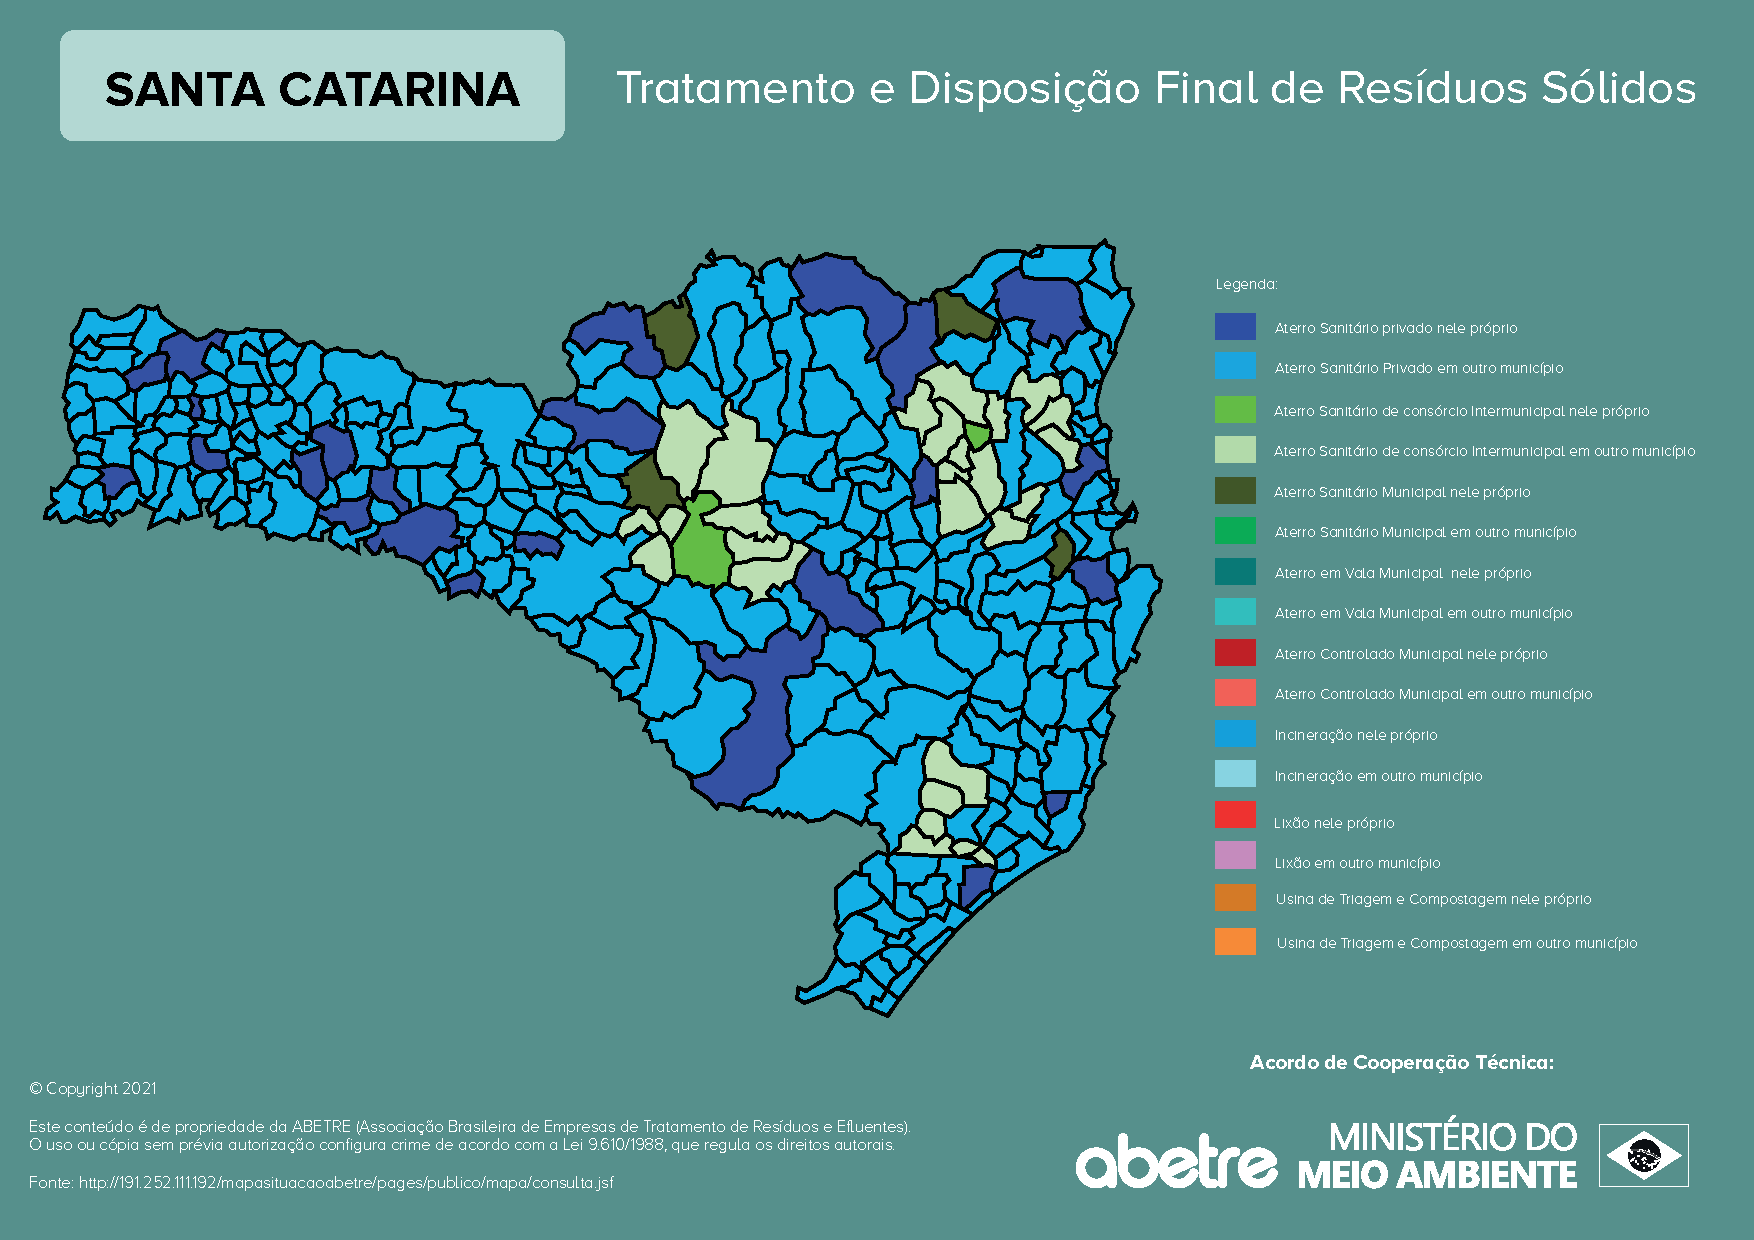
\includegraphics[scale=0.52]{images/abetre_sc.pdf}
	\end{center}
	\fonte{\gls{ABETRE}}
\end{figure}

\pagebreak
% ----------------------------------------------------------
\subsubsection{Aterro}
% ----------------------------------------------------------

Uma das destinações mais comuns no país, são áreas de armazenamento de resíduos \cite{diagnostico_cristine}:
\begin{itemize} 
	\item \textbf{Lixão:} a céu aberto;
	\item \textbf{Aterros Controlados:} em locais sem impermeabilização do solo;
	\item \textbf{Aterros Sanitários:} em espaço com engenharia dedicada à maior compactação dos resíduos e menor dano possível ao meio ambiente;
\end{itemize}
% ----------------------------------------------------------
\subsubsection{Tratamentos térmicos}
% ----------------------------------------------------------
Bastante utilizados no ramo da saúde \cite{diagnostico_cristine}:
\begin{itemize} 
	\item \textbf{Autoclave:} consiste na desinfecção dos resíduos através do aquecimento a uma temperatura elevada em contato com o vapor de água superaquecido;
	\item \textbf{Incineração:} queima dos resíduos a temperaturas superiores a 1000 °C numa atmosfera com oxigênio;
	\item \textbf{Microondas:} exposição dos resíduos à radiação eletromagnética de alta frequência;
	\item \textbf{Pirólise:} realiza-se o aquecimento dos materiais acima de 1000 °C numa atmosfera sem oxigênio;
\end{itemize}

% ----------------------------------------------------------
\subsubsection{Blendagem e coprocessamento}
% ----------------------------------------------------------

A \textbf{blendagem} é um processo de mistura de resíduos (\textit{"blends"}) a fim de gerar um produto alternativo ou matéria prima. Geralmente são misturados resíduos específicos para substituir ou reduzir o uso de uma matéria prima, barateando o processo. 

O \textbf{coprocesamento} utiliza os \textit{"blends"} de alto poder calorífico para destruição térmica dos resíduos em fornos de cimento resultando numa economia energética e de matéria prima \cite{noauthor_destinacao_nodate}


% ----------------------------------------------------------
\subsubsection{Compostagem}
% ----------------------------------------------------------

Trata-se de um método aeróbio de reciclagem e tratamento de resíduos orgânicos que busca reproduzir as condições observadas no processo natural de degradação da matéria orgânica \cite{diagnostico_cristine}.

% ----------------------------------------------------------
\subsubsection{Descontaminação de lâmpadas}
% ----------------------------------------------------------
Está relacionado à logística reversa das lâmpadas que contém mercúrio em sua composição. Consiste normalmente em pontos de entrega em estabelecimentos comerciais do país. As lampadas coletadas são transportadas e destinadas a recicladores homologados \cite{noauthor_legislacao_2023}.

% ----------------------------------------------------------
\subsubsection{Fins Didáticos}
% ----------------------------------------------------------

Trata da disposição de resíduos para utilização em unidades organizacionais. Por se tratar de uma movimentação de bem móvel entre organizações e órgãos da União fica regido pelo DECRETO Nº 10.340, 2020 \cite{brasil_decreto_2020}

% ----------------------------------------------------------
\subsubsection{Reciclagem} 
% ----------------------------------------------------------
De acordo com a \gls{PNRS}, reciclagem é o “processo de transformação dos resíduos sólidos que não seriam aproveitados, com mudanças em seus estados físico, físico-químico ou biológico, de modo a atribuir características ao resíduo para que ele se torne novamente matéria-prima ou novos produtos [...]” \cite[Art 3º, ítem XIV]{brasil_lei_nodate}.

% ----------------------------------------------------------
\subsubsection{Recuperação Energética}
% ----------------------------------------------------------

A recuperação energética é um processo que utiliza a energia contida nos resíduos sólidos para gerar eletricidade, calor ou combustíveis alternativos através da digestão anaeróbia, recuperação de gás de aterro sanitário, incineração e coprocessamento \cite{abren_abren_2021}

% ----------------------------------------------------------
\subsubsection{Rerrefino} 
% ----------------------------------------------------------

É o processo relacionado a recolhimento, coleta e destinação final de \gls{OLUC} de modo a aproveitar ao máximo seus constituintes e não causar danos ambientais \cite{diagnostico_cristine}.

% ----------------------------------------------------------
\subsubsection{Tratamento de Efluentes}
% ----------------------------------------------------------

Diz respeito à \gls{ETE}, que são: “unidades operacionais do sistema de esgotamento sanitário que através de processos físicos, químicos ou biológicos removem as cargas poluentes do esgoto, devolvendo ao ambiente o produto final,  efluente tratado, em conformidade com os padrões exigidos pela legislação ambiental.” \parencite{casan_ete_2023}

\subsubsection{Uso Agrícola}

É pertinente à utilização de resíduos como fertilizantes, sejam de origem agropecuária, urbana ou industrial. O uso de resíduos como fertilizantes atende requisitos da economia circular, economia verde e resíduo zero. \cite{diagnostico_cristine}


% ----------------------------------------------------------
\section{Classificações de resíduos sólidos industriais}
% ----------------------------------------------------------

A classificação de resíduos sólidos industriais é um processo fundamental que visa identificar suas características, riscos potenciais e formas apropriadas de tratamento e destinação. 

% ----------------------------------------------------------
\subsection{ABNT NBR 10004:2004}
% ----------------------------------------------------------

Para efeitos da norma ABNT NBR 10004:2004 Resíduos Sólidos — Classificação \cite{abnt_abnt_2004}, os resíduos são classificados com base no seu risco ao meio ambiente e à saúde. Os códigos possuem uma letra e três números. A classicação pode ser encontrada no \autoref{qua:Quadro_1}

\begin{quadro}[htb]
	\centering
	\caption{\label{qua:Quadro_1} Classificação de Resíduos Sólidos de acordo com a ABNT NBR 10004:2004}	
	\resizebox{\textwidth}{!}
	{\begin{tabular}{|l|p{11cm}|}
		\hline
		\textbf{Resíduos classe I — Perigosos} & São aqueles que em detrimento das características físicas, químicas e biológicas apresentam riscos a saúde e meio ambiente.  \\ \hline
		\textbf{Resíduos classe II — Não perigosos}        & São resíduos que não apresentam periculosidade aparente, exemplos são: sucatas, madeira, papel e papelão, borracha, areia de fundição, bagaço de cana.\\ \hline
		\textbf{Resíduos classe II A — Não inertes}          & São os resíduos que não se encaixam na classe II B. \\ \hline
		\textbf{Resíduos classe II B — Inertes}        & Quaisquer resíduos que, segundo normas auxiliares (ABNT NBR 10007 e ABNT NBR 10006) não tiverem nenhum de seus constituintes solubilizados e concentrações superiores aos padrões de potabilidade de água, excetuando-se aspecto, cor, turbidez, dureza e sabor. \\ \hline
	\end{tabular}}
	\fonte{\textcite{abnt_abnt_2004}.}
\end{quadro}


% ----------------------------------------------------------
\subsection{CONAMA}
% ----------------------------------------------------------

A RESOLUÇÃO CONAMA nº 358, 2005 \cite{noauthor_legislacao_conama_2005} com vistas a preservar a saúde pública e a qualidade do meio ambiente, dispõe sobre o tratamento e a disposição final dos resíduos dos serviços de saúde e dá outras providências, como a classificação dos resíduos em cinco grupos (A, B, C, D e E), conforme \autoref{qua:Quadro_2}

\begin{quadro}[htb]
	\centering
	\caption{\label{qua:Quadro_2} Classificação de Resíduos Sólidos de acordo com a CONAMA}	
	\resizebox{\textwidth}{!}{\begin{tabular}{|l|p{11cm}|}
		\hline
		\textbf{I — Grupo A} & Resíduos com a possível presença de agentes biológicos que, por suas características de maior virulência ou concentração, podem apresentar risco de infecção.  \\ \hline
		\textbf{II — Grupo B}        & Resíduos contendo substâncias químicas que podem apresentar risco à saúde pública ou ao meio ambiente, dependendo de suas características de infl amabilidade, corrosividade, reatividade e toxicidade\\ \hline
		\textbf{III — Grupo C}          &  Quaisquer materiais resultantes de atividades humanas que contenham radionuclídeos em quantidades superiores aos limites de eliminação especifi cados nas normas da Comissão Nacional de Energia Nuclear-CNEN e para os quais a reutilização é imprópria ou não prevista. \\ \hline
		\textbf{IV — Grupo D}        & Resíduos que não apresentem risco biológico, químico ou radiológico à saúde ou ao meio ambiente, podendo ser equiparados aos resíduos domiciliares. \\ \hline
		\textbf{V — Grupo E}        & Materiais perfurocortantes ou escarifi cantes, tais como: lâminas de barbear, agulhas, escalpes, ampolas de vidro, brocas, limas endodônticas, pontas diamantadas, lâminas de bisturi, lancetas; tubos capilares micropipetas; lâminas e lamínulas; espátulas; e todos os utensílios de vidro quebrados no laboratório (pipetas, tubos de coleta sanguínea e placas de Petri) e outros similares. \\ \hline
	\end{tabular}}
	\fonte{\textcite{noauthor_legislacao_conama_2005}.}
\end{quadro}

% ----------------------------------------------------------
\subsection{IBAMA}
% ----------------------------------------------------------

O \gls{IBAMA} por meio da INSTRUÇÃO NORMATIVA Nº 13, 2012 \cite{noauthor_instrucao_ibama} define que “A classificação de resíduos sólidos envolve a identificação do processo ou atividade que lhes deu origem, de seus constituintes e características, e a comparação destes constituintes com listagens de resíduos e substâncias cujo impacto à saúde e ao meio ambiente é conhecido.”.

Trata-se da classificação mais completa no Brasil até o momento de publicação desse trabalho, é também a referência para o \gls{MTR}. A estrutura segue um padrão de capítulo, subcapítulo, indicador de periculosidade e resíduo, consolidando no fim o código do resíduo, conforme \autoref{fig:Fig_2}. Atualmente, existe um total de 878 códigos classificando os resíduos sólidos; existe uma lista disponível no \href{https://www.gov.br/ibama/pt-br/assuntos/emissoes-e-residuos/residuos/arquivos?b_start:int=0}{\textbf{site do IBAMA}} nos formatos \href{https://www.gov.br/ibama/pt-br/assuntos/emissoes-e-residuos/residuos/arquivos/ibama-lista-brasileira-de-residuos-solidos.xls/view}{\textbf{.xls}} e \href{https://www.gov.br/ibama/pt-br/assuntos/emissoes-e-residuos/residuos/arquivos/ibama-lista-brasileira-de-residuos-solidos.doc/view}{\textbf{.doc}}

\begin{figure}[h]
	\caption{\label{fig:Fig_2} Exemplo de construção do código de identificação de resíduo do IBAMA}
	\begin{center}
		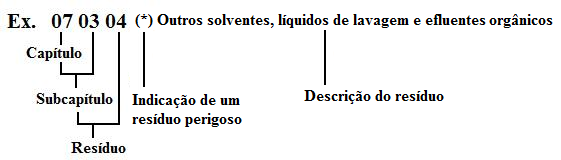
\includegraphics[scale=0.8]{images/exemplo-codigo-ibama.png}
	\end{center}
	\fonte{\gls{IBAMA}}
\end{figure}


% ----------------------------------------------------------
\section{Principais atividades industriais de SC}
% ----------------------------------------------------------

Para se obter um panorama sobre as atividades industriais que mais contribuem economicamente para o estado foi utilizado a \gls{PIA} - Empresa, o qual é elaborado uma vez por ano pelo \gls{IBGE} e investiga informações sobre as características estruturais básicas do segmento empresarial da atividade industrial no País, tendo como unidade de investigação a empresa industrial formalmente constituída cuja principal fonte de receita seja a atividade industrial \cite{ibge_pia-empresa_2021}. 

A pesquisa realiza o levantamento de diversas informações econômico-financeiras, como: receitas bruta e líquida; valor da transformação industrial; número de empresas e de unidades locais; pessoal ocupado; gastos com pessoal; custos de operação industrial, entre outros aspectos. 

Para os fins deste tópico, considerou-se dados gerais de empresas industriais com 5 ou mais pessoas ocupadas em \gls{SC} em 2021, e no momento o \gls{PIA} abrange apenas os \gls{CNAE} que compreendem as Indústrias Extatrivas e Indústrias de Transformação.

Na \autoref{fig:pia_it} é possível observar a predominância da indústria de fabricação de “Produtos alimentícios”, que em conjunto com as indústrias de “Máquinas, aparelhos e materiais elétricos”, “Confecção de artigos de vestuário e acessórios”, “Produtos têxteis”, "Máquinas e Equipamentos” e “Metalurgia” compõem mais de 60\% do \gls{VTI} das Indústrias de Transformação, o restante se divide em diversos outros setores, com destaque para os pontuados no gráfico. 

\begin{figure}[ht]
	\caption{\label{fig:pia_it} \gls{VTI} por grupo da Indústria de Transformação em \gls{SC} }
	\begin{center}
		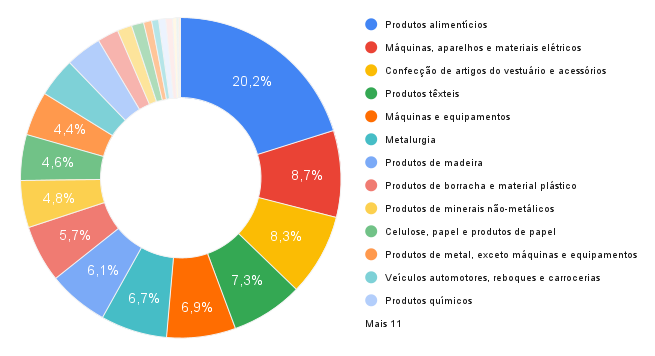
\includegraphics[scale=0.5]{images/pia-ibge-2021-it.png}
	\end{center}
	\fonte{Adaptado das tabelas do \textcite{ibge_pia-empresa_2021}}
\end{figure}

A Indústria Extrativa divide aproximadamente 1,5\% do \gls{VTI} com a Indústria de Transformação, sendo marjoritariamente composta pelas indústrias de “Carvão Mineral”, “Pedra, areia e argila” e “Outros minerais não-metálicos”, conforme ilustrado na \autoref{fig:pia_ie}.

\begin{figure}[ht]
	\caption{\label{fig:pia_ie} \gls{VTI} por grupo da Indústria Extrativa em \gls{SC} }
	\begin{center}
		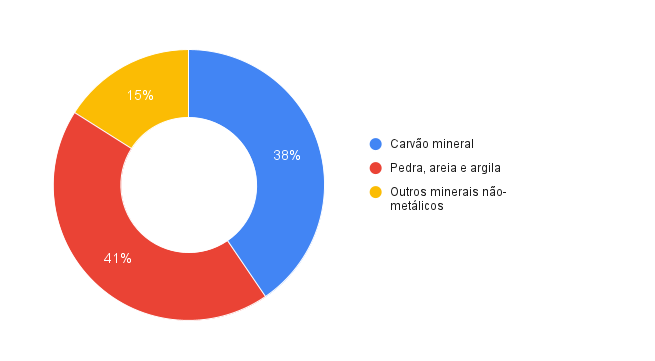
\includegraphics[scale=0.6]{images/pia-ibge-2021-ie.png}
	\end{center}
	\fonte{Adaptado das tabelas do \textcite{ibge_pia-empresa_2021}}
\end{figure}

% ----------------------------------------------------------
\section{Coleta de dados sobre resíduos sólidos industriais no Brasil}
% ----------------------------------------------------------

Na Era da Informação, já somos uma sociedade movida a dados, onde as tomadas de decisões são fundamentadas em evidências e informações coletadas por meio de análises e processamento de uma grande quantidade de dados (Big Data) \cite{castells_information_2010}. 

É notável que uma boa gestão de dados permite que tenhámos um melhor entendimento dos processos, e diante disso, reconhece-se a importância da coleta de dados sobre os resíduos sólidos no país para criação de políticas, práticas e ações que promovam o desenvolvimento sustentável, proteção do meio ambiente e melhoria da qualidade de vida da população, sendo um fator imprescíndivel nos dias atuais na tomada de decisão orientada a dados.

No Brasil, tem-se conhecimento de três principais fontes de dados sobre a geração e destinação de resíduos sólidos, estas são abordadas nas subseções.
% ----------------------------------------------------------
\subsection{MTR}
% ----------------------------------------------------------

Instituído pela portaria Portaria nº 280, de 29 de junho de 2020 \cite{mma_portaria_202}, o \gls{MTR} é uma ferramenta de gestão e documento de declaração nacional de implantação e operacionalização do \gls{PGRS}; a portaria dispõe que:

\begin{citacao}
	A utilização do MTR é obrigatória em todo o território nacional, para todos os geradores de resíduos sujeitos à elaboração de Plano de Gerenciamento de Resíduos Sólidos, conforme disposto no art. 20 da Lei nº 12.305, de 2 de agosto de 2010, que instituiu a Política Nacional de Resíduos Sólidos, como ferramenta online capaz de rastrear a massa de resíduos, controlando a geração, armazenamento temporário, transporte e destinação dos resíduos sólidos no Brasil. \cite[Art. 2º]{mma_portaria_202}
\end{citacao}

É base mais completa em nível de informações de rastreio de resíduos sólidos no âmbito nacional, e utiliza a lista de códigos de resíduos sólidos do \gls{IBAMA} para identificação dos resíduos.

O sistema é englobado ao \gls{SINIR} e requer um cadastro para que os envolvidos possam publicar o \gls{MTR}, sendo possível cadastrar tanto com o \gls{CPF} quanto com o \gls{CNPJ}. Como uma prática estadual estão sendo incorporados ao sistema do \gls{IMA} de cada \gls{UF}, requerindo também um cadastro para prosseguir. Na \autoref{fig:envio-mtr}, ilustra-se a aba de cadastro de manifesto no \href{http://mtr.ima.sc.gov.br/}{\textbf{site de MTR}} do \gls{IMA/SC}.

\begin{figure}[htb]
	\caption{\label{fig:envio-mtr} Janela de cadastro de \gls{MTR} do \gls{IMA/SC} }
	\begin{center}
		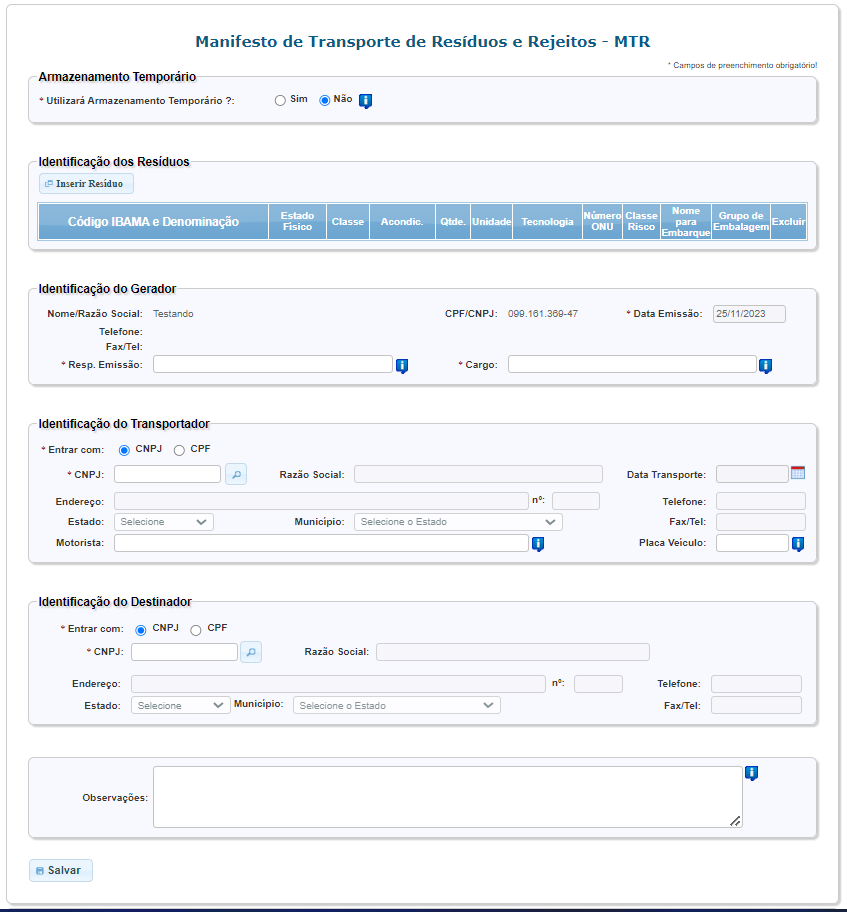
\includegraphics[scale=0.6]{images/envio-mtr.png}
	\end{center}
	\fonte{Captura de tela gerada pelo Autor (2023)}
\end{figure}

Para efeitos deste trabalho, foram feitas buscas pelos dados nas plataformas de dados abertos do \gls{MMA}, \gls{IBAMA}, \gls{IMA/SC} e do Governo Federal, mas infelizmente os dados não estão acessíveis publicamente até o momento da publicação deste trabalho. Fez-se necessário contactar o \gls{IMA/SC} para solicitação dos dados.



% ----------------------------------------------------------
\subsection{RAPP}
% ----------------------------------------------------------

O \gls{RAPP} faz parte do \gls{CTF/APP}, no qual todas pessoas jurídicas cadastradas, isolada ou cumulativamente, nas atividades constantes dos da Lei 6.938/1981 para as quais é obrigatório o preenchimento do formulário do \gls{RAPP}, conforme expresso nos Anexos I a XXVI da Instrução Normativa IBAMA n°06/2014. 

O relatório apresenta a relação de geradores de resíduos sólidos por Município/UF e por atividade cadastrada, descrição do resíduo gerado, quantidade, ano de geração e classificação de periculosidade. É a base mais completa no que diz respeito à quantidade de dados, contudo a classificação de resíduos é bastante ampla, por ex.: “Resíduos domiciliares”, “Resíduos Industriais”, “Resíduos da Construção Civil”.

Os dados estão acessíveis publicamente na plataforma de dados abertos do \href{https://dadosabertos.ibama.gov.br/organization/ibama?q=res%C3%ADduos&sort=score+desc%2C+metadata_modified+desc}{\textbf{IBAMA}} e também na do \href{https://dados.gov.br/dados/busca?termo=res%25C3%25ADduos%2520s%25C3%25B3lidos}{\textbf{Governo Federal}}.


% ----------------------------------------------------------
\subsection{Programa Nacional Lixão Zero}
% ----------------------------------------------------------


O Programa Nacional Lixão Zero é uma iniciativa da Secretaria de Qualidade Ambiental para implementar a \gls{PNRS}, integrando-se à Agenda Nacional de Qualidade Ambiental Urbana. O objetivo principal é apoiar estados e municípios na gestão adequada dos resíduos sólidos urbanos, com ênfase na disposição final ambientalmente correta. \cite{mma_programa_2019}

O programa dispõe \href{https://www.gov.br/mma/pt-br/acesso-a-informacao/acoes-e-programas/agendaambientalurbana/lixao-zero/Painel}{\textbf{painéis interativos no site}} que permitem a visualização de mapas, gráficos e indicadores relacionados à gestão de resíduos sólidos urbanos e logística reversa. No que tange aos dados, trata-se de uma base bastante completa em termos de informações,identificação dos resíduos e quantidade de dados; já utiliza os códigos de resíduos sólidos do \gls{IBAMA}.


% ----------------------------------------------------------
\subsection{SINIR}
% ----------------------------------------------------------

O \gls{SINIR} é um instrumento da \gls{PNRS} sob a responsabilidade do Governo Federal, por meio do \gls{MMA}. Com objetivo de unificar os dados sobre resíduos sólidos provenientes de diversas fontes, como o \gls{MTR}, \gls{RAPP}, \gls{SNIS}, \gls{IBGE}. No intuito de criar uma visualização integrada dessas bases o \gls{SINIR}+ compõe uma plataforma tecnológica para apoio à formulação de políticas públicas, em nível nacional, estadual e municipal, permitindo a gestão continuada de resíduos sólidos, além da criação de estratégias e oportunidades de negócios \cite{sinir_sinir_nodate}.

A plataforma é composta de mapas, painéis e relatórios que sistematizam os dados das fontes envolvidas e disponibilizam estatísticas e indicadores referentes à gestão de resíduos sólidos no Brasil. Apesar da plataforma do \gls{SINIR}+ integrar os dados em mapas e relatórios, e conforme mencionado no site que “[...] Professores e estudantes podem navegar em busca de informações gerais sobre os territórios em estudo, comparando regiões e entendendo os diferentes modelos de gestão empregados [...]” não foram encontrados arquivos de dados abertos em formatos que possibilitam uma análise mais específica da situação, por exemplo em \gls{CSV} ou \gls{JSON}.

A \autoref{fig:sinir-mapa} ilustra a visualização de mapa interativo disponibilida pelo \gls{SINIR}+ que permite a aplicação de camadas sob o mapa, permitindo visualizar correlações entre a geração/destinação de resíduos e infraestrutura urbana, por exemplo.

\begin{figure}[htb]
	\caption{\label{fig:sinir-mapa} Mapa interativo de Gestão de Resíduos Sólidos do \gls{SINIR}+}
	\begin{center}
		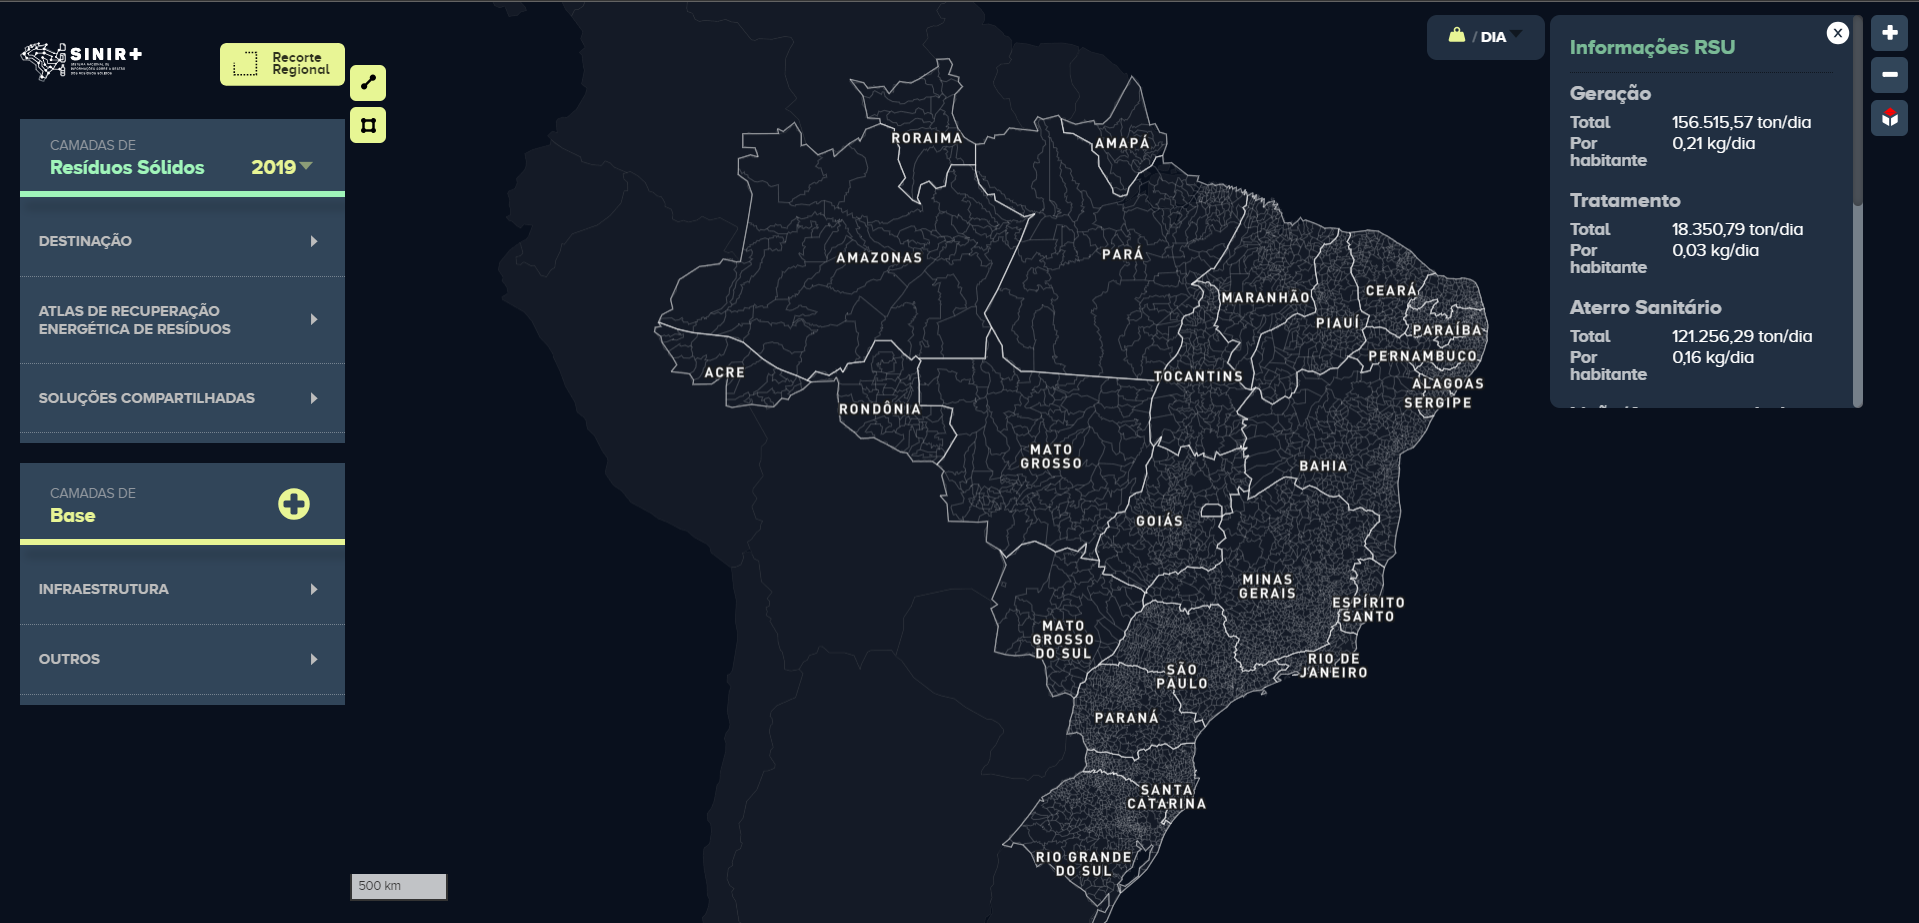
\includegraphics[scale=0.3]{images/sinir-mapa.png}
	\end{center}
	\fonte{Captura de tela gerada pelo Autor (2023)}
\end{figure}

\pagebreak

% ----------------------------------------------------------
\section{Economia Circular}
% ----------------------------------------------------------
A economia circular é um conceito que visa transformar o modelo econômico tradicional linear, baseado na extração, produção, consumo e descarte, em um modelo mais sustentável, que permita repensar as práticas econômicas da sociedade atual e que se inspira no funcionamento da própria Natureza \cite{leitao_economia_2015}. Neste quadro de desenvolvimento, os produtos possuem um ciclo fechado, protegendo e provendo ao meio ambiente, enquanto trabalha em parelelo com a intenção de compra e valor de mercado.

Neste cenário, englobando o pensamento de berço-a-berço (\textit{“Cradle to Cradle”}) \cite{braungart_cradle_2009}, há a oportunidade de fomentar o surgimento de novas dinâmicas entre as empresas, que passam de geradoras de resíduos numa cadeia produtiva, para consumidoras e fornecedoras de materiais num ciclo produtivo. 


% ----------------------------------------------------------
\section{Estado da arte}
% ----------------------------------------------------------

No contexto do gerenciamento de resíduos, existem muitos produtos surgindo para sanar uma lacuna no mercado e auxiliar empresas a melhorar a gestão da informação. Podemos citar os sistemas de gerenciamento “\href{https://www.meuresiduo.com/}{\textbf{meuResíduo}}” e “\href{https://www.resitrack.com.br/}{\textbf{Resitrack}}”, que com propostas bastante semelhantes permitem a unificação do controle de resíduos em um só lugar, substituindo as plataformas do Governo por uma ferramenta mais completa, que automatiza todo o processo de gestão da geração, armazenamento, transporte e destinação integrando com o sistema de \gls{MTR}.

No que diz respeito a uma plataforma de reinserção ou redirecionamento de resíduos no ciclo produtivo, podemos mencionar a “\href{https://www.cataki.org/}{\textbf{Cataki}}”, “\href{https://www.instagram.com/reciclae/}{\textbf{Reciclaê}}” e “\href{https://www1.sfiec.org.br/fiec-noticias/search/134129/sindiverde-lanca-app-que-conecta-produtores-de-residuos-a-industrias-de-reciclagem}{\textbf{Coleta Verde}}”, todos conectando a pessoas ou empresas geradoras a indústrias de reciclagem associadas. Ainda nesse âmbito, podemos mencionar a startup “\href{https://www.urupe.eco.br/}{\textbf{urupê}}”, que com uma proposta de gestão e consultoria realiza todo o processo relacionado a resíduos, visando garantir o maior aproveitamento dos resíduos.

Outra proposta, é a “\href{https://www.bubuyog.com.br/}{\textbf{bubuyog}}”, autonomeada \textit{“Tinder do Aço”}, que com uma plataforma estilo “\textit{marketplace}” auxilia as indústrias do ramo de aço a venderem produtos que, por algum motivo, ficaram parados nos estoques.